\chapter{Lec 21 - Autoencoders}

\section{Autoencoder - General Idea}
Autoencoders (AEs) are an unsupervised learning technique based on feed forward neural networks. The aim of autoencoders is to learn a representation (often called encoding or code) for a set of data, typically for the purpose of dimensionality reduction.\newline\newline
In particular, an autoencoder is a neural network that is trained to attempt to copy its input to its output.  Internally, it has a hidden layer $\textbf{h}$ that describes a code used to represent the input. The network may be viewed as consisting of two parts:
\begin{itemize}
    \item An \textbf{encoder} function $\textbf{h} = f(\textbf{x})$
    \item A \textbf{decoder} function that produces a reconstruction $\textbf{r} = g(\textbf{h})$
\end{itemize}
Since it is not useful to learn the identity function on the whole input domain (hidden code dimension equal to input dimension), autoencoders are trained to learn $\textbf{x} = g(f(\textbf{x}))$ with constraints:
\begin{itemize}
    \item on the architecture of the network (\textbf{undercomplete autoencoder}).

    \item adding a regularizing term to the loss (\textbf{overcomplete autoencoder})
\end{itemize}
Usually they are restricted in ways that allow them to copy only approximately. Because the model is forced to prioritize which aspects of the input should be copied, it often learns \textbf{useful properties} of the data.\newline\newline
Modern autoencoders have generalized the idea of an encoder and a decoder beyond deterministic functions to stochastic mappings $p_{encoder}(\textbf{h} | \textbf{x})$ and $p_{decoder}(\textbf{x} | \textbf{h})$. we may think of the decoder as providing a conditional distribution $p_{decoder}(\textbf{x} | \textbf{h})$. We may then train the autoencoder by minimizing $-log\, p_{decoder}(\textbf{x}|\textbf{h})$.

\section{Undercomplete Autoencoders}
One way to obtain useful features from the autoencoder is to constrain $\textbf{h}$ to have smaller dimension than $\textbf{x}$. An autoencoder whose code dimension is less than the input dimension is called \textbf{undercomplete}. Learning an undercomplete representation forces the autoencoder to capture the most salient features of the training data.\newline\newline
The learning process is described simply as minimizing a loss function;
\[L(\textbf{x}, g(f(\textbf{x}))\]
where $L$ is a loss function penalizing $g(f(\textbf{x}))$ for being dissimilar from $\textbf{x}$, such as the mean squared error.\newline\newline
When the decoder is linear and $L$ is the mean squared error, an undercomplete autoencoder learns to span the same subspace as \textbf{PCA} (SVD). Autoencoders with nonlinear encoder functions $f$ and nonlinear decoder functions $g$ can thus learn a more powerful nonlinear generalization of PCA. However, if the encoder and decoder are allowed too much capacity, the autoencoder can learn to perform the copying task without extracting useful information about the distribution of the data.\newline\newline
Autoencoders are often trained with only a single layer encoder and a single layer
decoder. However, this is not a requirement. In fact, using deep encoders and
decoders offers many advantages. Depth can exponentially reduce the computational cost of representing some functions. Depth can also exponentially decrease the amount of training data needed to learn some functions. Experimentally, \textbf{deep autoencoders} yield much better compression than corresponding shallow or linear autoencoders.

\subsection{Singular Value Decomposition (SVD)}
Singular Value Decomposition (SVD) is a standard linear dimensionality reduction method which combines the features of the original high-dimensional dataset and project them into a lower-dimensional space, ideally retaing most of their intrinsic properties.\newline\newline
Given a matrix $X$, the SVD decomposes it into the product of two unitary matrices, $V$ and $U$, and a rectangular diagonal matrix of singular values $S$:
\[X=V \cdot S \cdot U^T\]
The values in $S$ are called singular values. We can choose to keep only the first $k$ singular values in order to reduce the dimensionality of the input while minimizing the information loss.

\section{Overcomplete Autoencoders}
\textbf{Overcomplete} autoencoders have the hidden code dimension greater than the input. However, autoencoders may fail to learn useful properties of data if the dimension of the code $\textbf{h}$ is greater or equal to the input dimension. Therefore, rather than limiting the model capacity by keeping the encoder and decoder shallow and the code size small, \textbf{regularized autoencoders} use a loss function that encourages the model to have other properties besides the ability to copy its input to its output.\newline\newline
There are different types of regularized autoencoders:
\begin{itemize}
    \item Sparse autoencoders
    \item Denoising autoencoders 
    \item Contractive autoencoders
    \item Autoencoders with Dropout on the hidden layer
\end{itemize}

\section{Sparse Autoencoders}
A sparse autoencoder limits the capacity of the model by adding a sparsity penalty $\Omega(\textbf{h})$ on the code layer $\textbf{h}$, to the cost function:
\[L(\textbf{x}, g(f(\textbf{x}))) + \Omega(\textbf{h})\]
The sparsity penalty makes the model able to perform feature selection. In this way, a sparse autoencoder does not learn just the identity function, but it can learn useful features of the input.\newline\newline
Rather than thinking of the sparsity penalty as a regularizer for the copying task, we can think of the entire sparse autoencoder framework as approximating maximum likelihood training of a generative model that has latent variables (see slides for more details).

\section{Denoising Autoencoders}
Traditionally, autoencoders minimize some function:
\[L(\textbf{x}, g(f(\textbf{x})))\]
A \textbf{denoising autoencoder} or DAE instead minimizes:
\[L(\textbf{x}, g(f(\Tilde{\textbf{x}})))\]
where $\Tilde{\textbf{x}}$ is is a copy of $\textbf{x}$ that has been corrupted by some form of noise. Basically, DAE are forced to reconstruct a corrupted representation of the input. Denoising autoencoders must therefore undo this corruption rather than simply copying their input.\newline\newline
Like many other machine learning algorithms, autoencoders exploit the idea
that data concentrates around a low-dimensional \textbf{manifold}. Autoencoders aim to learn the structure of the manifold.
\begin{center}
    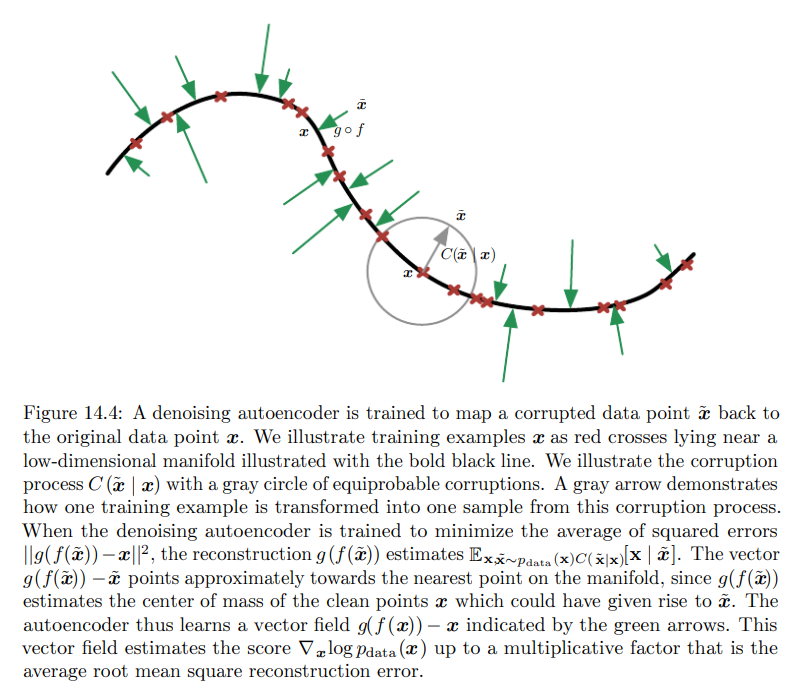
\includegraphics[scale=0.6]{images/manifold.png}
\end{center}

\section{Contractive Autoencoders}
The \textbf{contractive autoencoder} introduces an explicit regularizer on the code $\textbf{h} = f(\textbf{x})$, encouraging the derivatives of $f$ to be as small as possible:
\[\Omega(\textbf{h}) = \lambda ||\frac{\partial f(\textbf{x})}{\partial \textbf{x}}||^2_F\]
The penalty $\Omega(\textbf{h})$ is the squared Frobenius norm (sum of squared elements) of the Jacobian matrix of partial derivatives associated with the encoder function.\newline\newline
This forces the model to learn a function that does not change much when $\textbf{x}$ changes slightly.

